%%%%%%%%%%%%%%%%%%%%%%%%%%%%%%%% FIXED 
\documentclass[11pt]{article}
\usepackage{graphicx}
\pagestyle{empty}
\setlength{\parskip}{0.25\baselineskip}
\renewcommand{\title}[1]{{\noindent\large\bfseries#1\medskip\\}}
\renewcommand{\author}[2]{{\noindent #1 \medskip\\ \small #2 \medskip\\}}
\usepackage[letterpaper,margin=20mm]{geometry}
%%%%%%%%%%%%%%%%%%%%%%%%%%%%%%%%

\begin{document}

\title{Title of the submission to CCS 2025 Siena - Italy}
\author{
% Authors Names
First Author,\textsuperscript{1}
Second Author,\textsuperscript{2}
Third Author,\textsuperscript{3}
}
{
% Authors Affiliations
1. Address 1\\
2. Address 2\\
3. Address 3
}

% ABSTRACT
This is a short summary of the research that should take no more than a page [1].

This paper [2] delves into the intricate dynamics of networked human behavior within the context of complex systems, presenting a comprehensive exploration of the underlying mechanisms that govern interactions within social networks. As the digital age continues to redefine the landscape of human connectivity, understanding the complexities inherent in social systems becomes paramount. The research adopts an interdisciplinary approach, drawing insights from sociology, psychology, and network science to unravel the intricate interplay of factors shaping collective human behavior.

The study employs advanced computational models to analyze large-scale datasets obtained from diverse social platforms, shedding light on the emergent patterns that characterize human interactions. By integrating social network analysis with behavioral psychology frameworks, the research seeks to identify and quantify the factors influencing information diffusion, opinion formation, and the propagation of innovations within online and offline social networks.

Furthermore, the paper explores the impact of external stimuli, such as technological advancements and global events, on the evolution of social systems. It investigates how changes in network structures and individual behaviors can trigger cascading effects, leading to the emergence of novel phenomena within the complex fabric of human society.

The findings of this research have significant implications for a wide range of fields, including policy-making, marketing, and public health. Understanding the dynamics of networked human behavior enables the development of more effective strategies for targeted interventions, crisis management, and the promotion of positive societal change. The paper concludes with a discussion on the ethical considerations associated with the manipulation of social systems, emphasizing the need for responsible and transparent practices in an increasingly interconnected world.

This contribution to the Conference on Complex Systems 2024 aims to stimulate dialogue among researchers, practitioners, and policymakers, fostering a deeper understanding of the intricate nature of social systems and paving the way for innovative approaches to address the challenges and opportunities presented by the ever-evolving dynamics of human behavior in networked environments.

\bigskip
{\small
\noindent[1] Here you can add references.\\
\noindent[2] Differently from this one, not written using a LLM.
}

\begin{figure}[b]
  \centering
  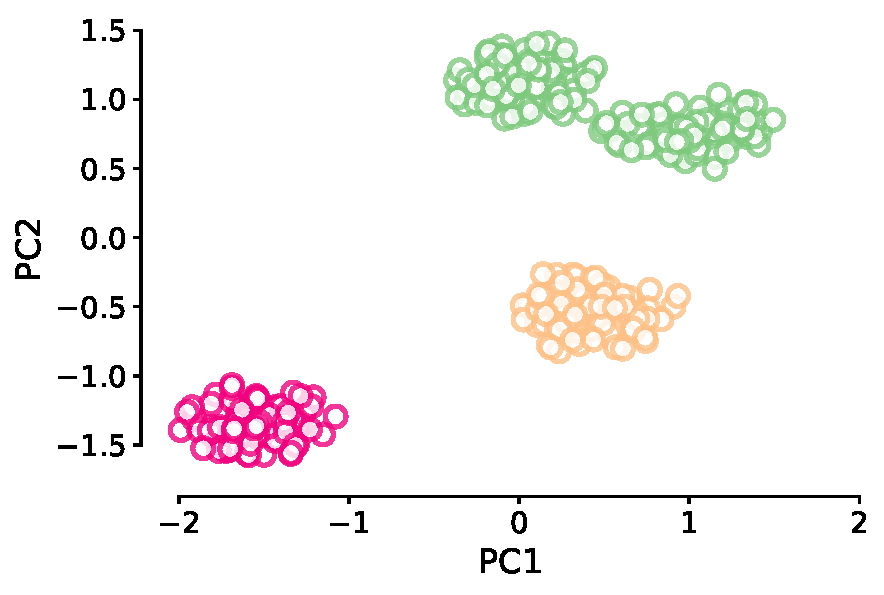
\includegraphics[width=0.5\textwidth]{figure.pdf}
  \caption{Figure caption.}
\end{figure}


\end{document}